%%%%%%%%%%%%%%%%%%%%%%%%%%%%%%%%%%%%%%%%%
% Beamer Presentation
% LaTeX Template
% Version 1.0 (10/11/12)
%
% This template has been downloaded from:
% http://www.LaTeXTemplates.com
%
% License:
% CC BY-NC-SA 3.0 (http://creativecommons.org/licenses/by-nc-sa/3.0/)
%
%%%%%%%%%%%%%%%%%%%%%%%%%%%%%%%%%%%%%%%%%

%----------------------------------------------------------------------------------------
%	PACKAGES AND THEMES
%----------------------------------------------------------------------------------------

\documentclass{beamer}

\mode<presentation> {

% The Beamer class comes with a number of default slide themes
% which change the colors and layouts of slides. Below this is a list
% of all the themes, uncomment each in turn to see what they look like.

%\usetheme{default}
%\usetheme{AnnArbor}
%\usetheme{Antibes}
%\usetheme{Bergen}
%\usetheme{Berkeley}
%\usetheme{Berlin}
\usetheme{Boadilla}
%\usetheme{CambridgeUS}
%\usetheme{Copenhagen}
%\usetheme{Darmstadt}
%\usetheme{Dresden}
%\usetheme{Frankfurt}
%\usetheme{Goettingen}
%\usetheme{Hannover}
%\usetheme{Ilmenau}
%\usetheme{JuanLesPins}
%\usetheme{Luebeck}
%\usetheme{Madrid}
%\usetheme{Malmoe}
%\usetheme{Marburg}
%\usetheme{Montpellier}
%\usetheme{PaloAlto}
%\usetheme{Pittsburgh}
%\usetheme{Rochester}
%\usetheme{Singapore}
%\usetheme{Szeged}
%\usetheme{Warsaw}

% As well as themes, the Beamer class has a number of color themes
% for any slide theme. Uncomment each of these in turn to see how it
% changes the colors of your current slide theme.

%\usecolortheme{albatross}
%\usecolortheme{beaver}
%\usecolortheme{beetle}
%\usecolortheme{crane}
%\usecolortheme{dolphin}
%\usecolortheme{dove}
%\usecolortheme{fly}
%\usecolortheme{lily}
%\usecolortheme{orchid}
%\usecolortheme{rose}
%\usecolortheme{seagull}
%\usecolortheme{seahorse}
\usecolortheme{whale}
%\usecolortheme{wolverine}

%\setbeamertemplate{footline} % To remove the footer line in all slides uncomment this line
%\setbeamertemplate{footline}[page number] % To replace the footer line in all slides with a simple slide count uncomment this line

%\setbeamertemplate{navigation symbols}{} % To remove the navigation symbols from the bottom of all slides uncomment this line
}

\usepackage{graphicx} % Allows including images
\usepackage{booktabs} % Allows the use of \toprule, \midrule and \bottomrule in tables

%----------------------------------------------------------------------------------------
%	TITLE PAGE
%----------------------------------------------------------------------------------------

\title[Localization using RADAR]{Radar Based Vehicle Localization} % The short title appears at the bottom of every slide, the full title is only on the title page

\author[Awies \& Prathamesh]
{%
   \texorpdfstring{
        \begin{columns}
            \column{.45\linewidth}
            \centering
            Prathamesh Saraf\\
            A59015739\\
            \href{mailto:psaraf@ucsd.edu}{psaraf@ucsd.edu} 
            \column{.45\linewidth}
            \centering
            Awies Mohammad Mulla\\
            A59016119 \\
            \href{mailto:amulla@ucsd.edu}{amulla@ucsd.edu}
        \end{columns}
   }
   {Awies Mohammad Mulla \& Prathamesh Saraf}
}% Your name
\institute[UCSD] % Your institution as it will appear on the bottom of every slide, may be shorthand to save space
{
% Increase size of below text
\Large
\textbf{University of California, San Diego} \\ % Your institution for the title page
\medskip
}
\titlegraphic{
\includegraphics[scale=0.035]{ucsd.png}}
\date{December 11, 2023} % Date, can be changed to a custom date

\begin{document}

\begin{frame}
\titlepage % Print the title page as the first slide
\end{frame}

\begin{frame}
\frametitle{Overview} % Table of contents slide, comment this block out to remove it
\tableofcontents % Throughout your presentation, if you choose to use \section{} and \subsection{} commands, these will automatically be printed on this slide as an overview of your presentation
\end{frame}

%----------------------------------------------------------------------------------------
%	PRESENTATION SLIDES
%----------------------------------------------------------------------------------------
%------------------------------------------------
\section{Problem Formulation} % Sections can be created in order to organize your presentation into discrete blocks, all sections and subsections are automatically printed in the table of contents as an overview of the talk
%------------------------------------------------
\subsection{Problem Statement}
\begin{frame}
\frametitle{Problem Statement}
\begin{itemize}
    \item \textbf{Objective:} Estimate the position of a moving vehicle using data from two RADAR sensors.
    \item \textbf{Trajectory:} Non-linear, involving turns.
    \item \textbf{RADAR Locations:} 
        \begin{itemize}
            \item RADAR 1: $(0, 0)$
            \item RADAR 2: $(0, -1000)$
        \end{itemize}
    \item \textbf{Data:} Radar-derived cartesian coordinates $(x, y)$.
    \item \textbf{Road Map Context:} Information about the road intersections and turns.
    \item \textbf{Speed:} Nominal speed is known with increment standard deviation.
    \item \textbf{Goal:} Fuse the radar data along with road dynamics and speed for enhanced tracking.
\end{itemize}
\end{frame}

\subsection{System Dynamics}

\begin{frame}
\frametitle{System Dynamics}
\begin{itemize}
    \item The agent is assumed to be a point mass. Here, we have used two state space representations for the in-depth analysis of the problem.
    \item \textbf{State Space 1:}
    \begin{align*}
        \begin{bmatrix}
            x_{k+1} \\
            v^x_{k+1} \\
            y_{k+1} \\
            v^y_{k+1}
        \end{bmatrix} &= \begin{bmatrix}
            1 & \Delta t & 0 & 0 \\
            0 & 1 & 0 & 0 \\
            0 & 0 & 1 & \Delta t \\
            0 & 0 & 0 & 1
        \end{bmatrix}
        \begin{bmatrix}
            x_k \\
            v^x_k \\
            y_k \\
            v^y_k
        \end{bmatrix}
    \end{align*}
    \item \textbf{State Space 2:}
    \begin{align*}
        \begin{bmatrix}
            x_{k+1} \\
            y_{k+1} \\
        \end{bmatrix} &= \begin{bmatrix}
            1 & 0 \\
            0 & 1
        \end{bmatrix} \begin{bmatrix}
            x_k \\
            y_k
        \end{bmatrix} + \begin{bmatrix}
            \Delta t & 0 \\
            0 & \Delta t
        \end{bmatrix} \begin{bmatrix}
            v^x_k \\
            v^y_k
        \end{bmatrix}
    \end{align*}
\end{itemize}
\end{frame}
\begin{frame}
\frametitle{System Dynamics}
\begin{itemize}
    \item In one case velocity is used as the state variable and in the other case it is used as an input.
    \item We have used Constant Velocity Motion model with white noise acceleration. The standard deviations for the white noise accelerations were different for North-South path and East-West path.
    \item Standard Deviations for North-South path:
    \begin{align*}
        \sigma_{\Delta v_x} &= 1.18 \\
        \sigma_{\Delta v_y} &= 1.67
    \end{align*}
    \item Standard Deviations for East-West path:
    \begin{align*}
        \sigma_{\Delta v_x} &= 1.18 \\
        \sigma_{\Delta v_y} &= 0.83
    \end{align*}
    \item The Radar errors are known to be:
    \begin{align*}
        r &= 95 \ m \\
        \theta &= 0.0035 \ mr
    \end{align*}
    where $r$ is the range and $\theta$ is the bearing angle.
\end{itemize}
\end{frame}
%------------------------------------------------

\section{Tracking Algorithms}
\subsection{Averaging Filter}
\begin{frame}
\frametitle{Averaging Filter}
\begin{figure}
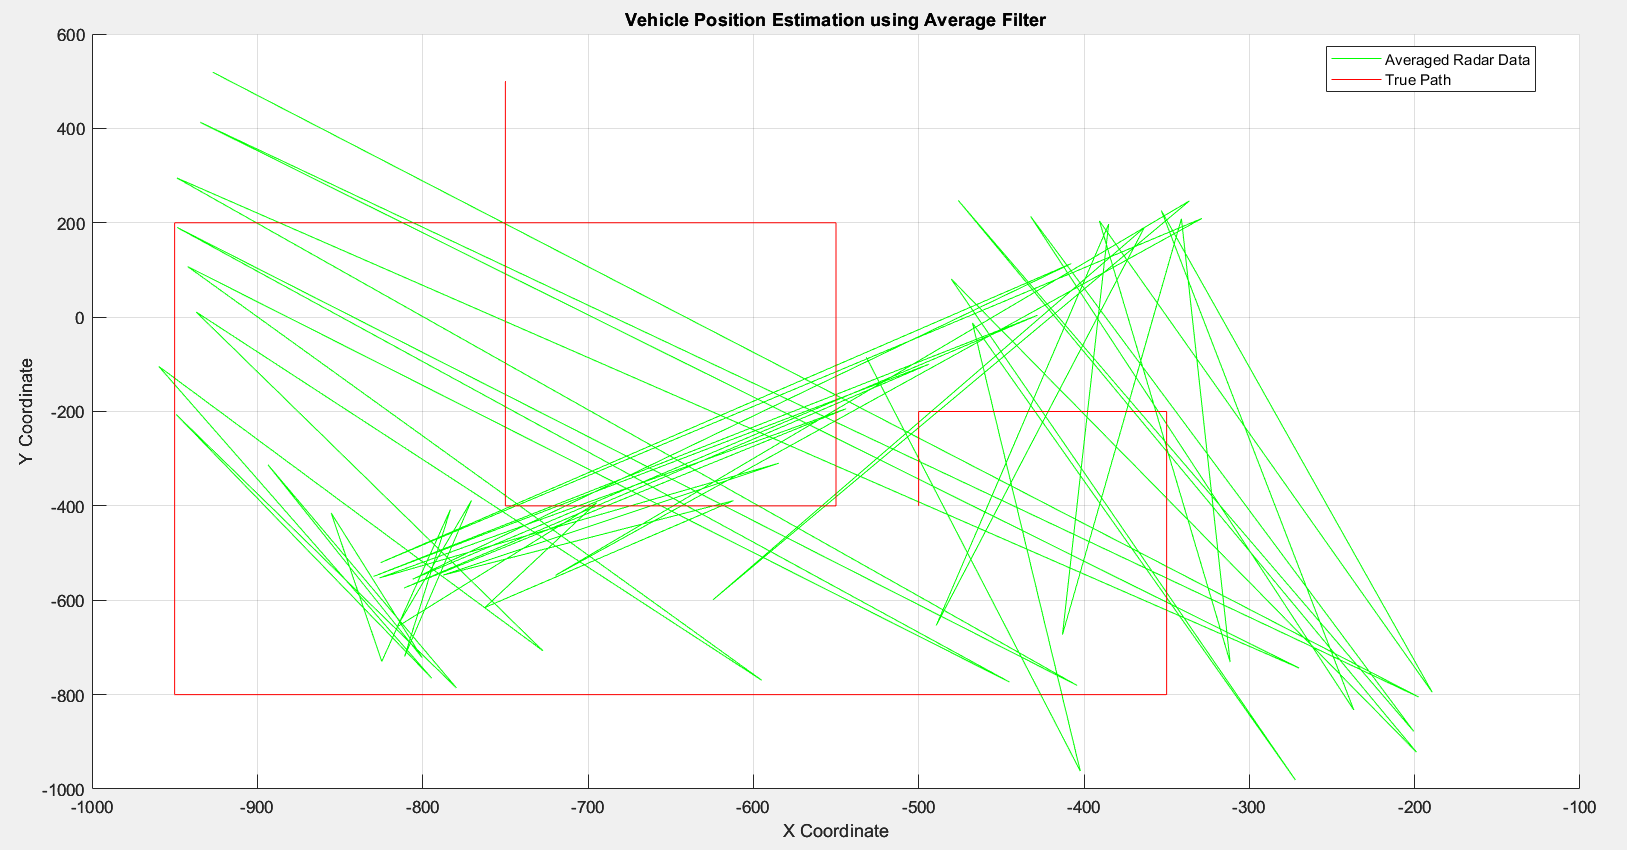
\includegraphics[width=0.65\linewidth]{avg_filter.png}
\end{figure}
The RADAR measurements representing the position of the agent are given in cartesian coordinates ($(x^1_t, y^1_t)$ and $(x^2_t, y^2_t)$). Resulting average filter estimate is given by:
\begin{equation*}
    x^{avg}_t = \frac{x^1_t + x^2_t}{2} \hspace*{1cm}
    y^{avg}_t = \frac{y^1_t + y^2_t}{2}
\end{equation*}
\end{frame}

\subsection{Alpha-Beta Filter}
\begin{frame}
\frametitle{Alpha-Beta Filter}
\begin{itemize}
    \item Using the state space representation 2 and the system dynamics, we can write the state space equations as:
    \begin{align*}
        \hat{\mathbf(x)}_k &\leftarrow A \hat{\mathbf(x)}_{k-1} + B \mathbf(u)_k + \frac{\Delta t^2}{2}\mathbf{w}_k \\
    \end{align*}
    where $\hat{\mathbf(x)}_k$ is the state estimate at time $k$, $\mathbf(u)_k$ is control input and $A$ and $B$ are the state transition and control matrices respectively. 
    $\mathbf{w}_k$ is the process noise which is $\mathbf{w}_k \sim \mathcal{N}(0, Q)$. $Q$ (white noise $\text{acc}^{\text{n}}$) is given by:
    \begin{align*}
        Q &= \begin{bmatrix}
            \sigma^2_{\Delta v_x} & 0 \\
            0 & \sigma^2_{\Delta v_y}
        \end{bmatrix}
    \end{align*}
\end{itemize}
\end{frame}

\begin{frame}
\frametitle{Alpha-Beta Filter}
\begin{itemize}
\item The output measurement is expected to deviate form prediction due to noise. So, the predcition error (residual) is given by:
\begin{align*}
    \mathbf{r}_k &= \mathbf{z}_k - \hat{\mathbf{x}}_k
\end{align*}
where $\mathbf{z}_k$ is the measurement vector from sensor which here is the RADAR measurement ($\mathbf{x}^{avg}_k$).
\item The alpha-beta filter corrects the estimated state using the residual as:
\begin{align*}
    \hat{\mathbf{x}}_k &\leftarrow \hat{\mathbf{x}_k} + \alpha \mathbf{r}_k \\
    \hat{\mathbf{v}}_k &\leftarrow \hat{\mathbf{v}_k} + \frac{\beta}{\Delta t} \mathbf{r}_k
\end{align*}
\end{itemize}
\end{frame}

\begin{frame}
\frametitle{Alpha-Beta Filter: Results and Analysis}
\begin{figure}
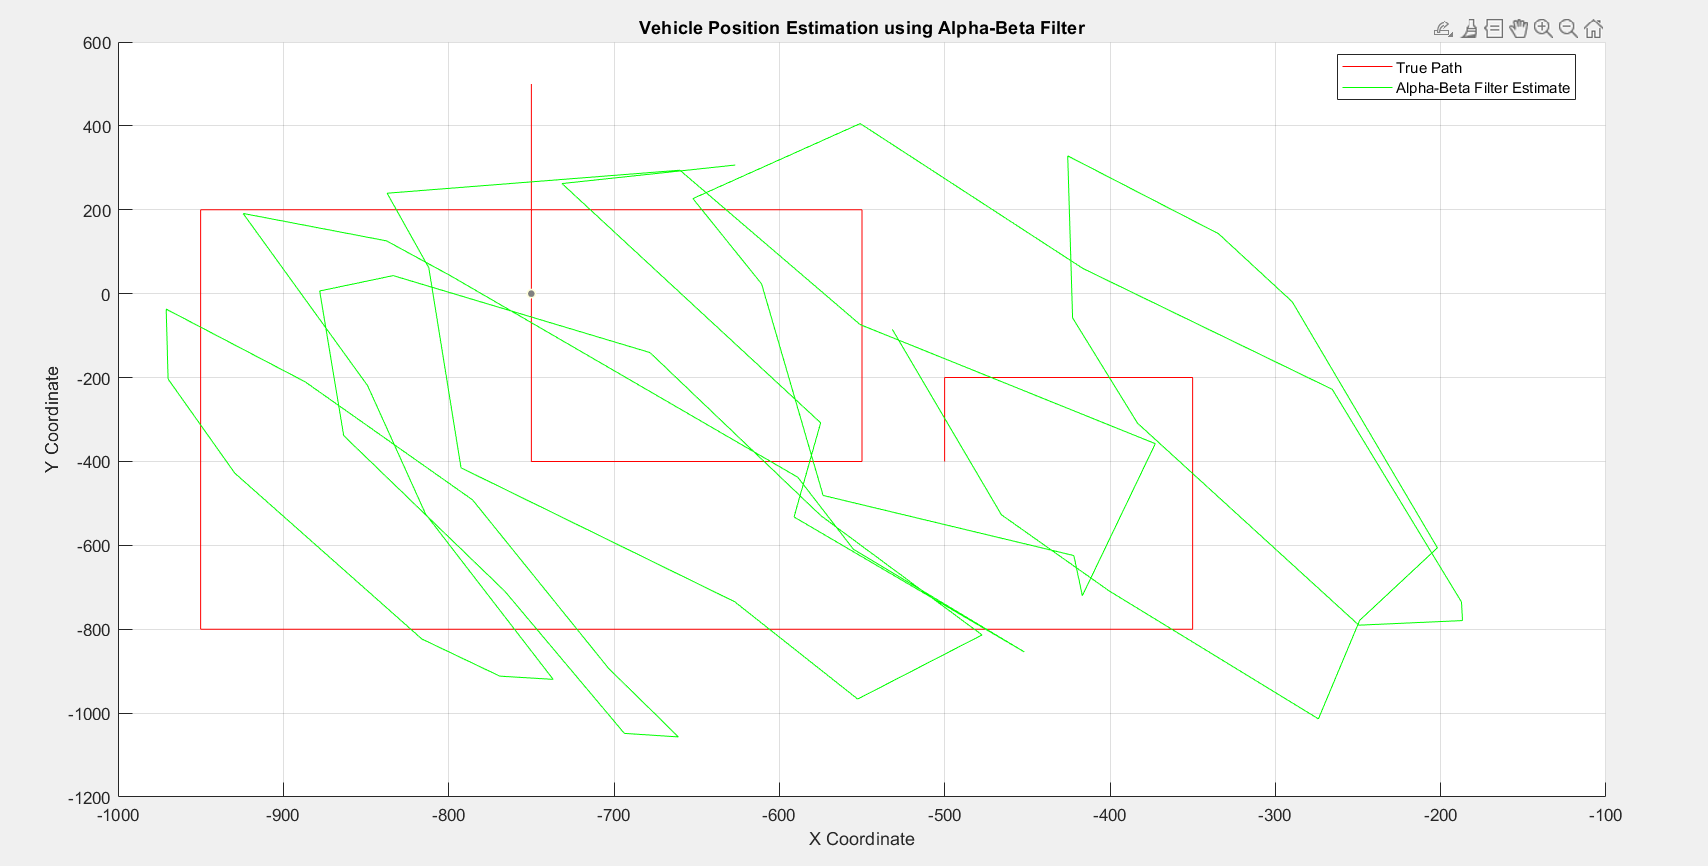
\includegraphics[width=0.65\linewidth]{alpha_beta.png}
\end{figure}
In general, larger $\alpha$ and $\beta$ gains tend to produce faster response for tracking transient changes, while smaller
$\alpha$ and $\beta$ gains reduce the level of noise in the state estimate.
\begin{equation*}
    \alpha = 0.5 \hspace*{1cm} \beta = 0.1
\end{equation*}
\end{frame}

\subsection{Kalman Filter}
\begin{frame}
\frametitle{Kalman Filter}
\begin{itemize}
    \item Kalman filter is a bayesian filter based on the fact that, system dynamics is linear and Markovian.
    \item The state of the system is represented by a Gaussian distribution with mean $\mu_k$ and covariance $P_k$.
    \item Here, we are following the state space representation 2 and the corresponding system dynamics. The motion model is given by:
    \begin{align*}
        \hat{\mathbf{x}}_k &\leftarrow A \hat{\mathbf{x}}_{k-1} + C \mathbf{w}_k
    \end{align*}
    where $\mathbf{w}_k$ is the process noise which is $\mathbf{w}_k \sim \mathcal{N}(0, Q)$. $A$ and $C$ are given by:
    \begin{equation*}
        A = \begin{bmatrix}
            1 & \Delta t & 0 & 0 \\
            0 & 1 & 0 & 0 \\
            0 & 0 & 1 & \Delta t \\
            0 & 0 & 0 & 1
        \end{bmatrix} \hspace{1cm} 
        C = \begin{bmatrix}
            \frac{\Delta t^2}{2} & 0 \\
            \Delta t & 0 \\
            0 & \frac{\Delta t^2}{2} \\
            0 & \Delta t
        \end{bmatrix}
    \end{equation*}
\end{itemize}
\end{frame}

\begin{frame}
\frametitle{Kalman Filter}
\begin{itemize}
    \item Observation model is given by:
    \begin{align*}
        \mathbf{z}_k &= H \hat{\mathbf{x}}_k + \mathbf{v}_k
    \end{align*}
    where $\mathbf{v}_k$ is the measurement noise which is $\mathbf{v}_k \sim \mathcal{N}(0, R)$. $H$ and $R$ are given by:
    \begin{equation*}
        H = \begin{bmatrix}
            1 & 0 & 0 & 0 \\
            0 & 0 & 1 & 0
        \end{bmatrix} \hspace{1cm} 
        R = \begin{bmatrix}
            \sigma^2_x & 0 \\
            0 & \sigma^2_y
        \end{bmatrix}
    \end{equation*}
    where $\sigma_x$ and $\sigma_y$ are the standard deviations of the RADAR measurements in cartesian coodinates calculated from 
    range and bearing angle errors.
\end{itemize}
\end{frame}

\begin{frame}
\frametitle{Kalman Filter}
\begin{itemize}
    \item The Kalman Filter is a two step process:
    \begin{enumerate}
        \item \textbf{Prediction:} Predict the state of the system at time $k$ using the motion model.
        \begin{align*}
            \mu_k^- &= A \mu_{k-1} \\
            P_k^- &= A P_{k-1} A^T + Q
        \end{align*}
        \item \textbf{Correction:} Correct the predicted state using the measurement model.
        \begin{align*}
            \mathbf{K}_k &= P_k^- H^T (H P_k^- H^T + R)^{-1} \\
            \mu_k &= \mu_k^- + \mathbf{K}_k (\mathbf{z}_k - H \mu_k^-) \\
            P_k &= (I - \mathbf{K}_k H) P_k^-
        \end{align*}
        where $\mathbf{K}_k$ is the Kalman Gain.
    \end{enumerate}
\end{itemize}
\end{frame}

\begin{frame}
\frametitle{Kalman Filter: Results}
\begin{figure}
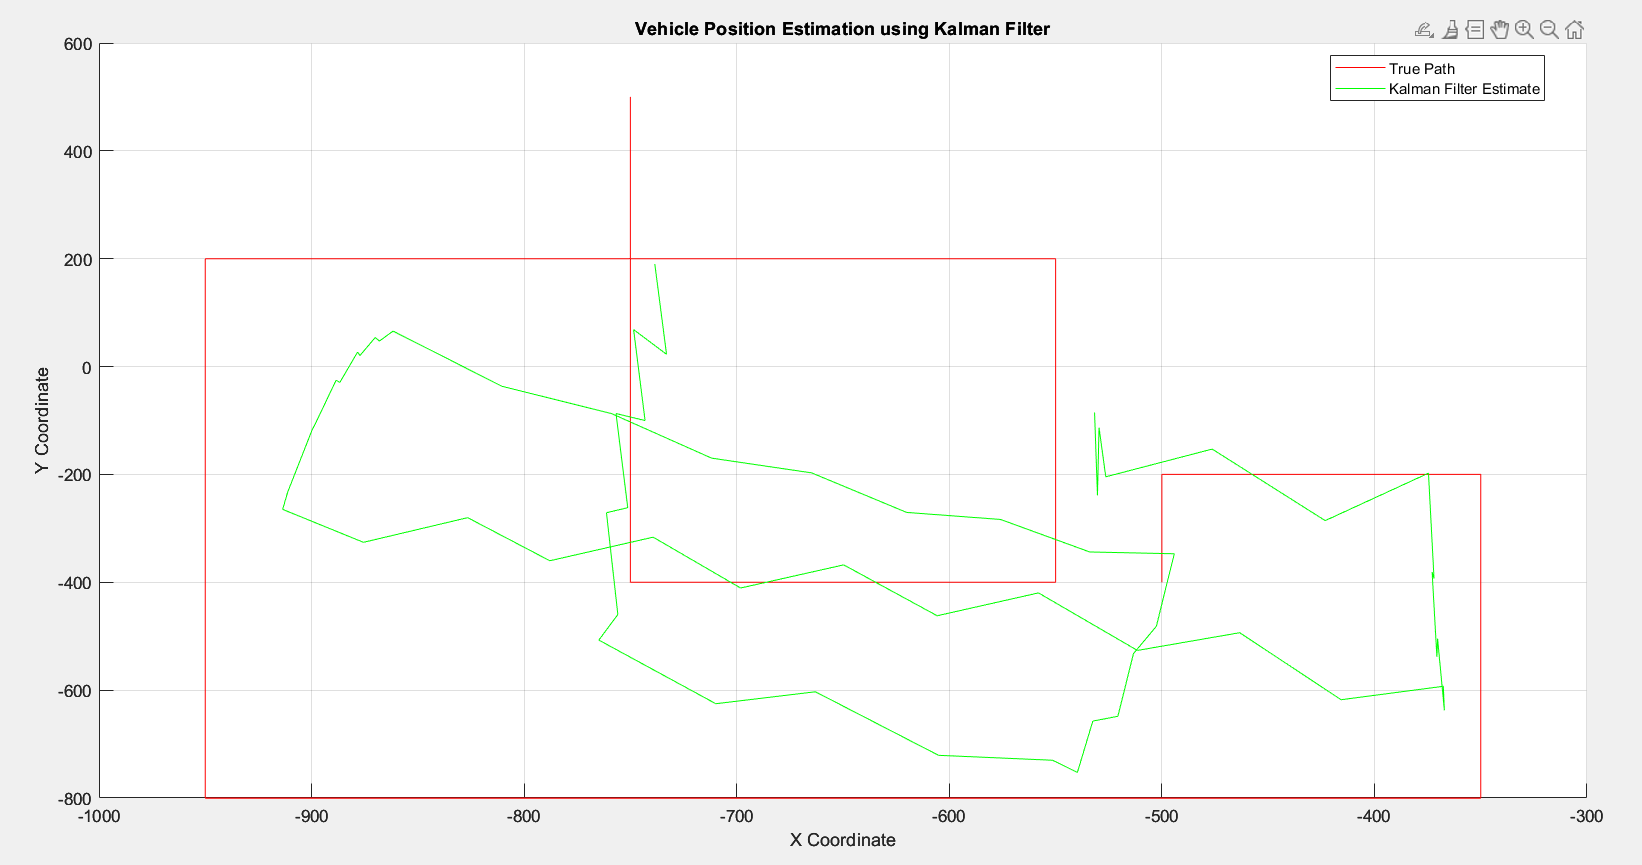
\includegraphics[width=0.8\linewidth]{kalman.png}
\end{figure}
\end{frame}

\subsection{Extended Kalman Filter}
\begin{frame}
\frametitle{Extended Kalman Filter}
\begin{itemize}
    \item The Extended Kalman Filter is used to deal with non-linear system dynamics. Here we are using the state space representation 1 and the corresponding system dynamics.
    \item The motion model is given by:
    \begin{align*}
        \hat{\mathbf{x}}_k &\leftarrow A \hat{\mathbf{x}}_{k-1} + B \mathbf{u}_k + \frac{\Delta t^2}{2}\mathbf{w}_k
    \end{align*}
    where, the notations are same as in the case of Kalman Filter and alpha-beta filter.
    \item The observation model is given by:
    \begin{align*}
        \mathbf{z}_k &= h(\hat{\mathbf{x}}_k, \mathbf{v}_k)
    \end{align*}
    where $h(\hat{\mathbf{x}}_k)$ is the non-linear observation model and $\mathbf{v}_k$ is the measurement noise which is $\mathbf{v}_k \sim \mathcal{N}(0, R)$. $R$ is given by:
    \begin{equation*}
        R = \begin{bmatrix}
            \sigma^2_r & 0 \\
            0 & \sigma^2_{\theta}
        \end{bmatrix}
    \end{equation*}
\end{itemize}
\end{frame}

\begin{frame}
\frametitle{Extended Kalman Filter}
\begin{itemize}
    \item The range and bearing angle errors are given by:
    \begin{align*}
        \sigma_r &= 95 m \\
        \sigma_{\theta} &= 0.035 radians
    \end{align*}
    \item Since, the non-linearity arise in the observation model for our case. We can linearize the observation model using Taylor series expansion.
    \item The linearized observation model is given by:
    \begin{align*}
        \mathbf{z}_k &= h(\hat{\mathbf{x}}_k, \mathbf{v}_k) \approx H(\hat{\mathbf{x}}_k) + \mathbf{v}_k
    \end{align*}
    where, $H$ is the Jacobian of the observation model.
    \item The Jacobian of the observation model is given by:
    \begin{align*}
        H &= \begin{bmatrix}
            \frac{\hat{x}_k}{\sqrt{\hat{x}_k^2 + \hat{y}_k^2}} & \frac{\hat{y}_k}{\sqrt{\hat{x}_k^2 + \hat{y}_k^2}} \\
            \frac{-\hat{y}_k}{\hat{x}_k^2 + \hat{y}_k^2} & \frac{\hat{x}_k}{\hat{x}_k^2 + \hat{y}_k^2}
        \end{bmatrix}
    \end{align*}
\end{itemize}
\end{frame}

\begin{frame}
\frametitle{Extended Kalman Filter: Results and Analysis}
\begin{figure}
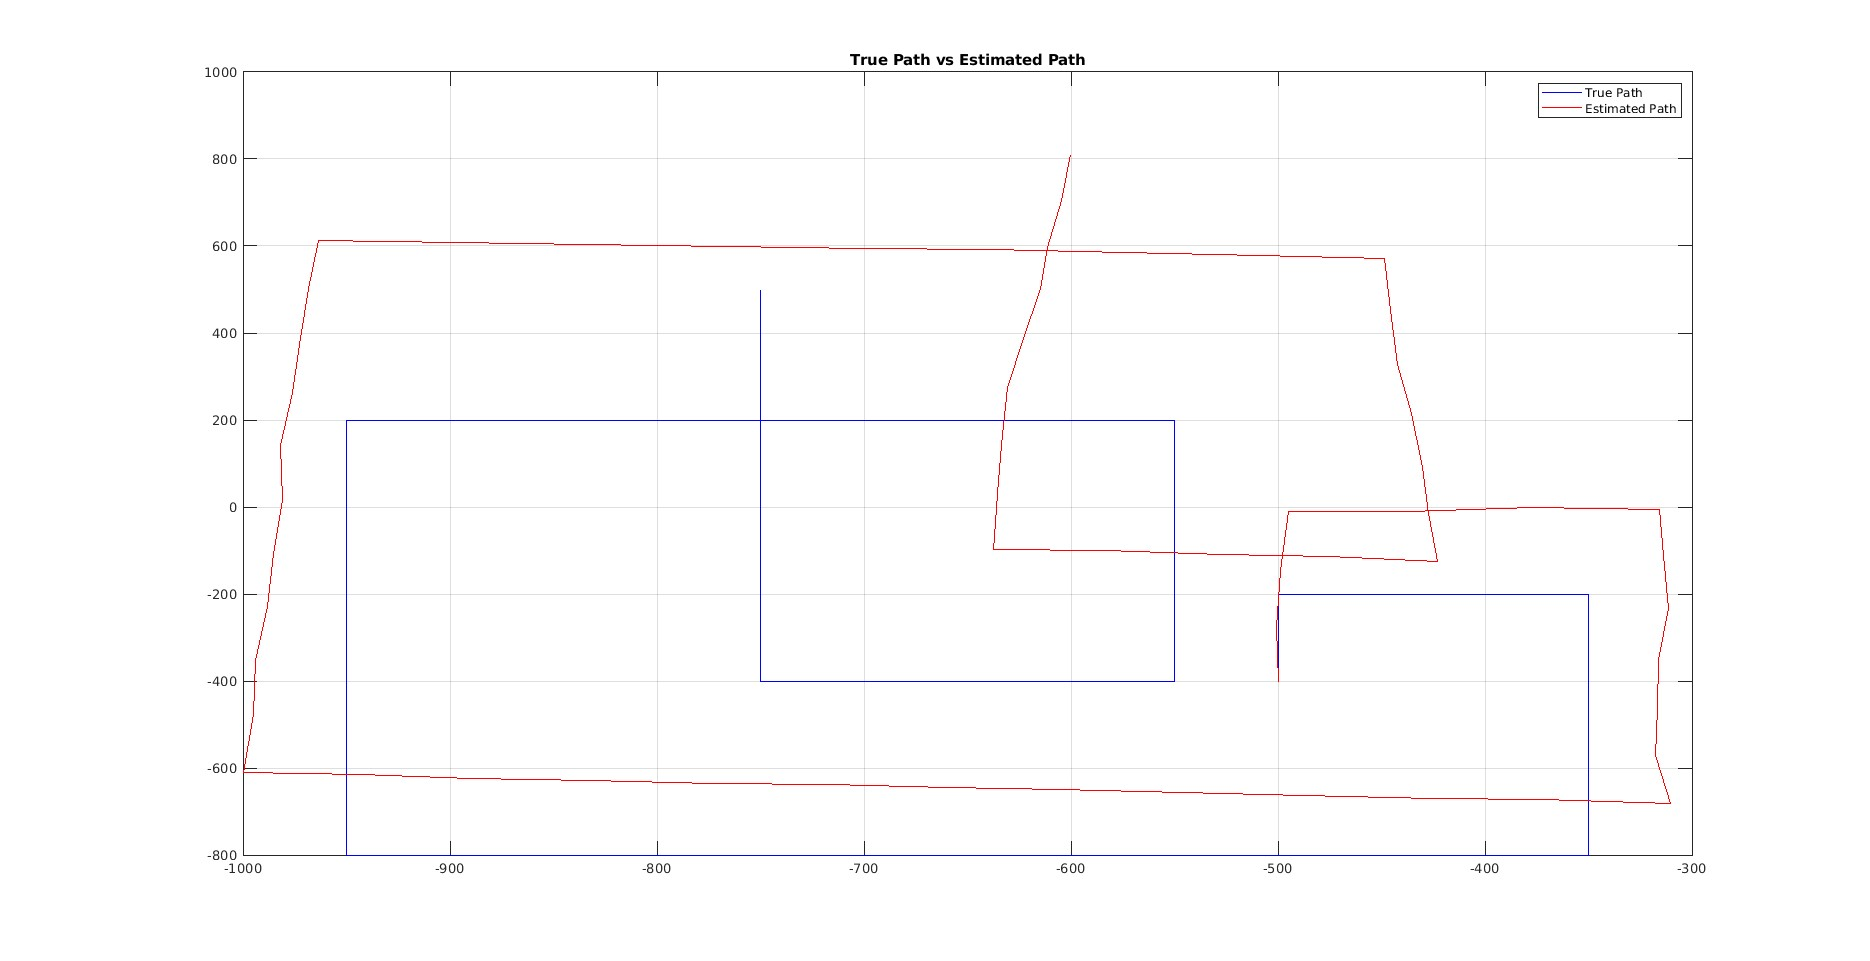
\includegraphics[width=0.9\linewidth]{ekf.jpg}
\end{figure}
Observed bias in the above plot is due to the error in the initial RADAR measurement.
\end{frame}

\subsection{Particle Filter}
\begin{frame}
\frametitle{Particle Filter}
\begin{itemize}
    \item Particle filter is a non-parametric implementation of the Bayes filter. Each particle represents a hypothesis of the state of the system.
    \item The state of the system is represented by a set of particles $\{\mathbf{x}^i_k\}_{i=1}^N$ with weights $\{w^i_k\}_{i=1}^N$.
    \item The motion model is given by:
    \begin{align*}
        \mathbf{x}^i_k &\leftarrow f(\mathbf{x}^i_{k-1}, \mathbf{u}_k) \\
        w^i_k &\leftarrow w^i_{k-1} p(\mathbf{z}_k | \mathbf{x}^i_k)
    \end{align*}
    \item The observation model is given by:
    \begin{align*}
        \mathbf{z}_k &= h(\mathbf{x}^i_k)
    \end{align*}
    \item The weights are normalized at each time step to take care of dying weights problem.
\end{itemize}
\end{frame}

% 2 column slide
\begin{frame}
\frametitle{Particle Filter: Illustration}
\begin{columns}[c] 
\column{.5\textwidth}
\begin{figure}
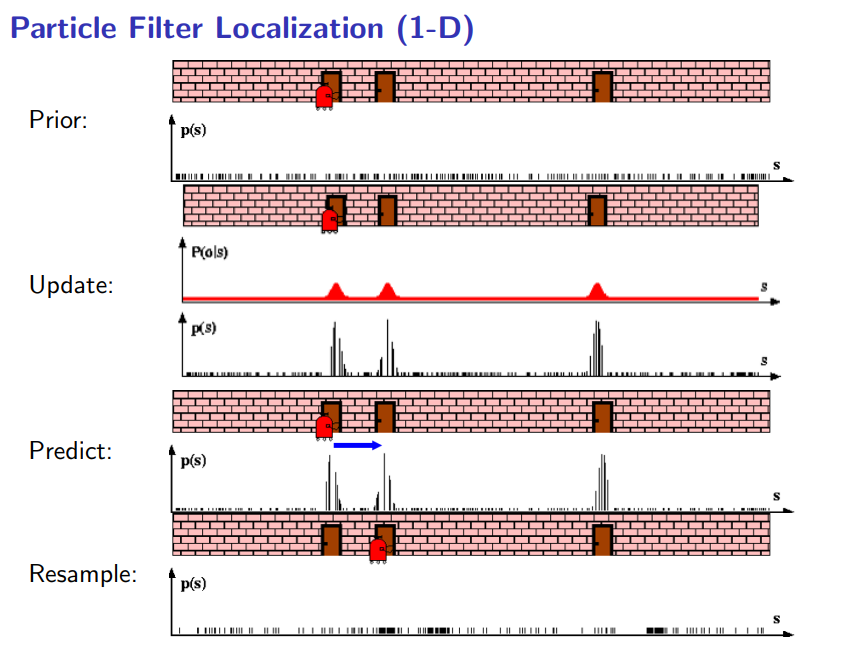
\includegraphics[width=1.0\linewidth]{PF_eg.png}
\end{figure}
\column{.5\textwidth} % Right column and width
\begin{figure}
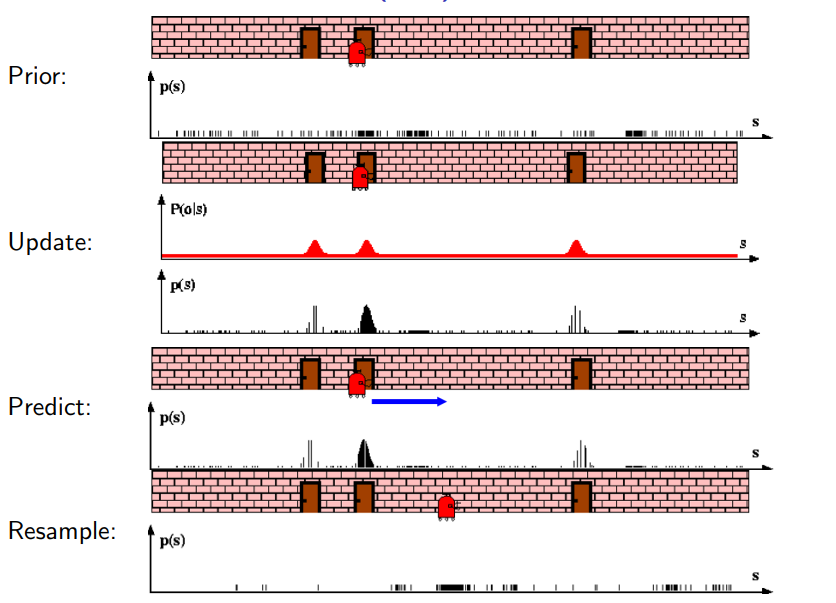
\includegraphics[width=1.0\linewidth]{PF_eg2.png}
\end{figure}
\end{columns}
\end{frame}

\begin{frame}
\frametitle{Particle Filter: Using True Velocities}
\begin{figure}
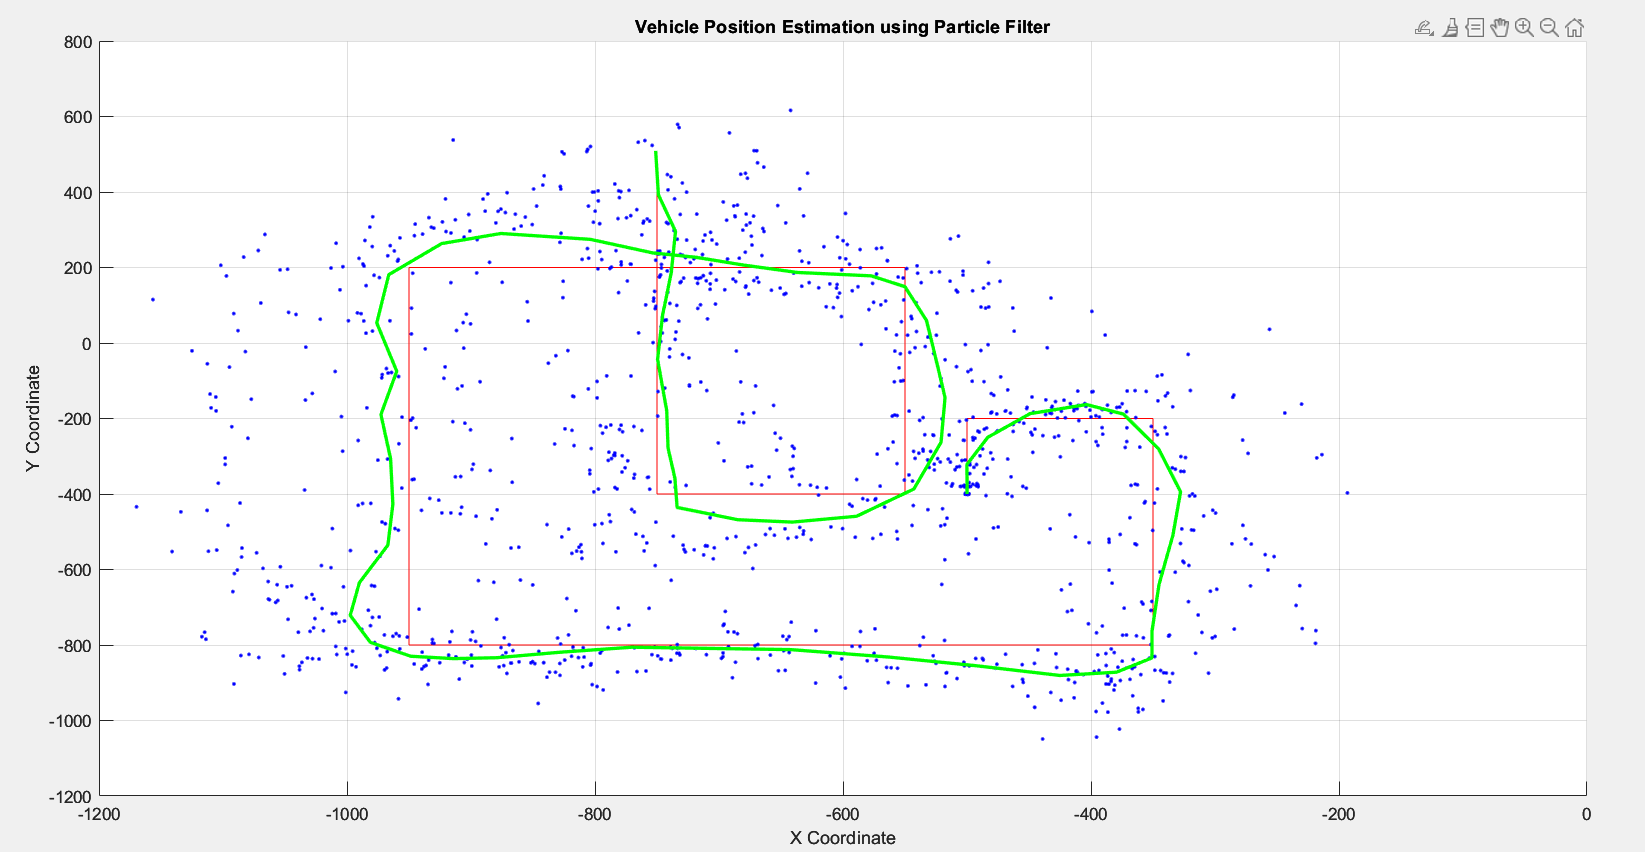
\includegraphics[width=1.0\linewidth]{PF_results.png}
\end{figure}
\end{frame}

\begin{frame}
\frametitle{Particle Filter: Using RADAR Velocities}
\begin{figure}
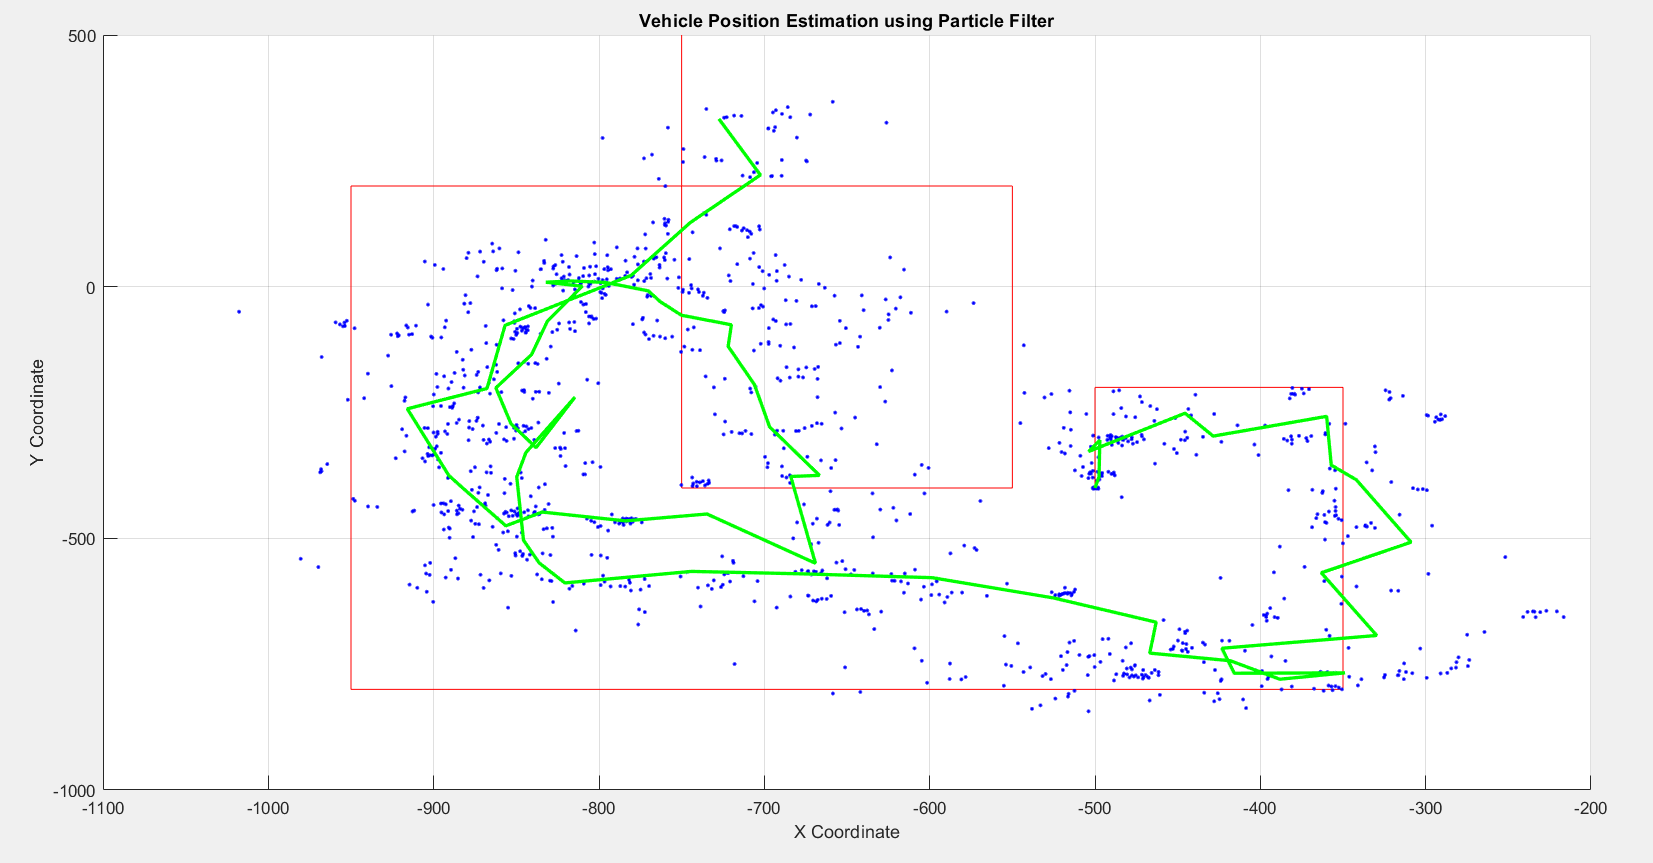
\includegraphics[width=1.0\linewidth]{PF_results2.png}
\end{figure}
\end{frame}

\section{Conclusion and Future Work}
\begin{frame}
\frametitle{Conclusion and Future Work}
\begin{itemize}
    \item The Kalman Filter and Extended Kalman Filter are the most efficient filters for tracking the agent.
    \item Since, the RADAR measurements are really skewed and noisy, the averaging and the alpha-beta filters are not able to track the agent properly.
    \item The particle filter is able to provide decent results as shown but not only is it computationally expensive but also we would need to use appropriate observation
    model to update the likelihood of the particles.
    \item In the future, we could drastically improve the results if we fuse the data from a sensor measuring velocity and heading of the agent. The heading of the agent could be estimated using the 
    IMU measurements.
    \item We were also trying to implement a piecewise Kalman Filter which would use the information from the map to reduce the covariance of the state estimate.
\end{itemize}
\end{frame}


%------------------------------------------------

\section{References}

%------------------------------------------------

\begin{frame}
\frametitle{References}
\footnotesize{
\begin{thebibliography}{99} % Beamer does not support BibTeX so references must be inserted manually as below
\bibitem[D.D. Sworder]{p1} D.D. Sworder (2007)
\newblock Assurance regions in tracking
\newblock \href{https://drive.google.com/file/d/1W1eB29tVJYWAzfcWRojw3QTsvRBPBr-w/view?usp=sharing}{\underline{link}}
\end{thebibliography}
\begin{thebibliography}{99} % Beamer does not support BibTeX so references must be inserted manually as below
    \bibitem[Baisa]{p2} Nathanel L. Baisa (2020)
    \newblock Derivation of Constant Velocity Motion Model for Visual Tracking
    \newblock \href{https://arxiv.org/pdf/2005.00844.pdf}{\underline{link}}
    \end{thebibliography}
}

\end{frame}

%------------------------------------------------

\begin{frame}
\Huge{\centerline{Thank You}}
\end{frame}

%----------------------------------------------------------------------------------------

\end{document}